\section{Results}

\subsection{Facility expansion and recorded activity growth}
Across the fixed-member comparisons, facility expansion is faster than recorded activity growth. In the 36-city cohort observed throughout 2019--2023, activity increases by \AChange\% while facilities increase by \NChange\%, so facility-weighted network intensity falls by \IDecline\%. This is a growth-rate gap, not a claim that activity falls everywhere: the same cohort includes cities with positive activity growth and cities with absolute contraction. The facility-weighted decomposition assigns \WithinChange{} index points to within-city intensity changes and \WeightChange{} to changing facility weights. The positive weight term offsets part of the within-city decline, so the network-wide movement cannot be reduced to a simple shift towards lower-intensity cities.

The result is not confined to the longest window. The four adjacent-year comparisons contain 39, 55, 77 and 93 cities; their intensity changes are negative in every case, including a \MiddleIDecline\% decline in 2020--2021 and a \RecentIDecline\% decline in 2022--2023. The three continuous three-year windows contain \ThreeEarlyN, \ThreeMiddleN{} and \ThreeLateN{} cities, with intensity declines of \ThreeEarlyDecline\%, \ThreeMiddleDecline\% and \ThreeLateDecline\%. These windows have different memberships and durations, so they show a recurring comparison across the available fixed supports rather than independent replications. Table~\ref{tab:growth_windows} gives the corresponding window estimates, while Figure~\ref{fig:growth} places the fixed 36-city path beside the network aggregates and equal-city distributions. Network-wide intensity changes are ratios of summed activity and facilities, whereas the distribution panels summarize equal-city log changes; the two operators answer related but distinct questions.

The broader endpoint frame tests whether the positive-only rule drives the direction of the result. In 2022--2023, 225 cities have finite endpoint activity, facilities and compatible-week measures. The 117 $00$ cities account for 52.00\% of the endpoint city count but only 3.47\% of endpoint facilities; the 93 $++$ cities account for 95.04\% of endpoint facilities. Across all 225 cities, activity grows 15.32\%, facilities grow 45.70\% and facility-weighted network intensity falls 20.85\%. Within the $++$ group, facilities grow 42.78\% and intensity falls 19.52\%, so the direction persists when the comparison is restricted to cities with positive activity at both endpoints, while the magnitude depends on the represented facility denominator. Table~\ref{tab:recorded_states} reports the state counts, aggregate changes and activity decomposition; SI Tables~\siref{tab:record_state_details} and \siref{tab:record_state_activity_details} give state-specific facility shares and endpoint levels.

The state decomposition identifies where the broad-set activity change comes from. The persistent-positive group contributes +14.907 baseline activity-index points, compared with +0.418 from $0+$, $-0.003$ from $+0$ and 0 from $00$. Thus state-changing cities remain part of the observation frame, but they make small signed contributions to the activity total in this endpoint comparison. These labels describe source-recorded endpoint states; they do not determine commissioning, entry into demand or service shutdown.
\begin{table}[htbp]\centering\small\caption{Recorded activity states and changes}\label{tab:recorded_states}
\begin{tabular}{@{}lrrrrr@{}}\toprule\multicolumn{6}{l}{Panel A: Recorded states by fixed common-city window}\\\midrule
Window & Cities & $++$ & $0+$ & $+0$ & $00$\\
\midrule
2019--2020 & 47 & 39 & 3 & 2 & 3\\
2020--2021 & 70 & 55 & 5 & 1 & 9\\
2021--2022 & 167 & 77 & 11 & 4 & 75\\
2022--2023 & 225 & 93 & 10 & 5 & 117\\
\bottomrule\end{tabular}
\par\medskip\begin{tabular}{@{}lrrr@{}}\toprule\multicolumn{4}{l}{Panel B: All-member percentage changes}\\\midrule
Window & $\Delta A$ (\%) & $\Delta N$ (\%) & $\Delta I$ (\%)\\
\midrule
2019--2020 & 7.67 & 35.91 & -20.78\\
2020--2021 & 44.82 & 46.72 & -1.30\\
2021--2022 & 3.84 & 45.29 & -28.53\\
2022--2023 & 15.32 & 45.70 & -20.85\\
\bottomrule\end{tabular}
\par\medskip\begin{tabular}{@{}lrrrrr@{}}\toprule\multicolumn{6}{l}{Panel C: Activity change contributions (percentage points; baseline activity = 100)}\\\midrule
Window & $++$ & $0+$ & $+0$ & $00$ & Total\\
\midrule
2019--2020 & 7.613 & 0.069 & -0.015 & 0.000 & 7.667\\
2020--2021 & 44.847 & 0.060 & -0.089 & 0.000 & 44.818\\
2021--2022 & 3.716 & 0.158 & -0.033 & 0.000 & 3.841\\
2022--2023 & 14.907 & 0.418 & -0.003 & 0.000 & 15.322\\
\bottomrule\end{tabular}\end{table}


\subsection{City growth patterns and transitions}
The common aggregate gap contains distinct city-level regimes. All 36 long-cohort cities expand facilities: \LongFast{} have faster activity growth and increasing intensity, \LongSlow{} have positive activity growth that is slower than facility growth, and \LongContract{} combine facility expansion with activity contraction. The slower-positive group is therefore a relative-pace result, whereas the contraction group also involves an absolute fall in activity. In the recent 2022--2023 window, the corresponding counts are \RecentFast{} faster-growth, \RecentSlow{} slower-positive and \RecentContract{} contraction cities, with \RecentOther{} boundary or nonexpansion cases. These are window-specific descriptions, not permanent city types or ordered development stages.

Initial facility scale does not supply a common trajectory. The 93 recent-window cities divide into three equal baseline-scale groups; their median log-intensity changes are \SizeLowI, \SizeMiddleI{} and \SizeHighI{} from low to high scale, with overlapping interquartile ranges. Spatial and scale comparisons retain the full recent membership, including five changes beyond the map's symmetric display limit. Cities with expanding facilities therefore occupy different positions relative to the equal-growth boundary, and baseline scale alone does not account for that variation (Figure~\ref{fig:regimes}).
\begin{table}[htbp]\centering\small\caption{Facility and activity growth}\label{tab:growth_windows}
\begin{tabular}{@{}lrrrrr@{}}\toprule\multicolumn{6}{l}{Panel A: Aggregate changes and city intensity directions}\\\midrule
Window & Cities & $\Delta A$ (\%) & $\Delta N$ (\%) & $\Delta I$ (\%) & $I$ declines: $n$ (\%)\\
\midrule
2019--2023 & 36 & 75.77 & 289.34 & -54.85 & 30 (83.3)\\
2019--2020 & 39 & 7.61 & 36.05 & -20.90 & 28 (71.8)\\
2020--2021 & 55 & 44.89 & 46.53 & -1.12 & 19 (34.5)\\
2021--2022 & 77 & 3.72 & 45.12 & -28.53 & 45 (58.4)\\
2022--2023 & 93 & 14.91 & 42.78 & -19.52 & 54 (58.1)\\
2019--2021 & 38 & 54.75 & 96.27 & -21.15 & 26 (68.4)\\
2020--2022 & 53 & 47.49 & 110.42 & -29.91 & 26 (49.1)\\
2021--2023 & 73 & 17.89 & 104.56 & -42.37 & 51 (69.9)\\
\bottomrule\end{tabular}
\par\medskip\begin{tabular}{@{}lrrrrr@{}}\toprule\multicolumn{6}{l}{Panel B: Growth-regime counts (percentage of window cities)}\\\midrule
Window & Cities & Faster & Slower & Contraction & Other\\
\midrule
2019--2023 & 36 & 6 (16.7) & 22 (61.1) & 8 (22.2) & 0 (0.0)\\
2019--2020 & 39 & 10 (25.6) & 10 (25.6) & 9 (23.1) & 10 (25.6)\\
2020--2021 & 55 & 28 (50.9) & 12 (21.8) & 4 (7.3) & 11 (20.0)\\
2021--2022 & 77 & 24 (31.2) & 25 (32.5) & 15 (19.5) & 13 (16.9)\\
2022--2023 & 93 & 38 (40.9) & 28 (30.1) & 25 (26.9) & 2 (2.2)\\
2019--2021 & 38 & 11 (28.9) & 15 (39.5) & 7 (18.4) & 5 (13.2)\\
2020--2022 & 53 & 23 (43.4) & 16 (30.2) & 8 (15.1) & 6 (11.3)\\
2021--2023 & 73 & 22 (30.1) & 32 (43.8) & 18 (24.7) & 1 (1.4)\\
\bottomrule\end{tabular}\end{table}

\begin{figure}[htbp]\centering
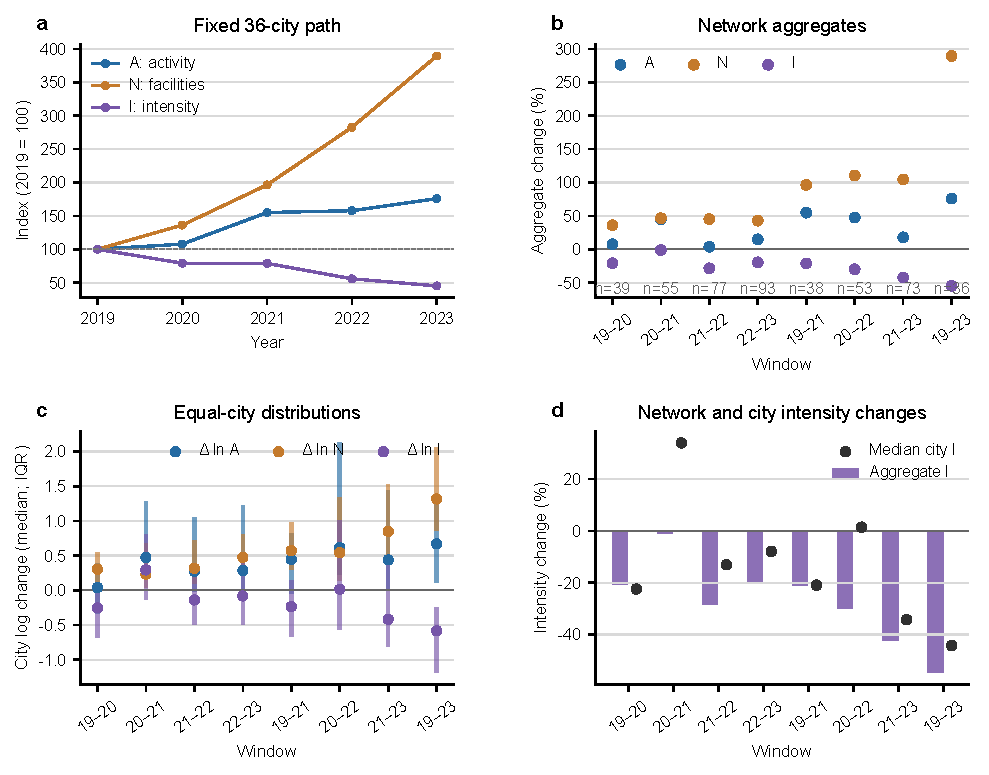
\includegraphics[width=\linewidth,height=.76\textheight,keepaspectratio]{figures/fig3_growth.pdf}
\caption{Facility and activity growth}\label{fig:growth}
\end{figure}

\begin{figure}[htbp]\centering
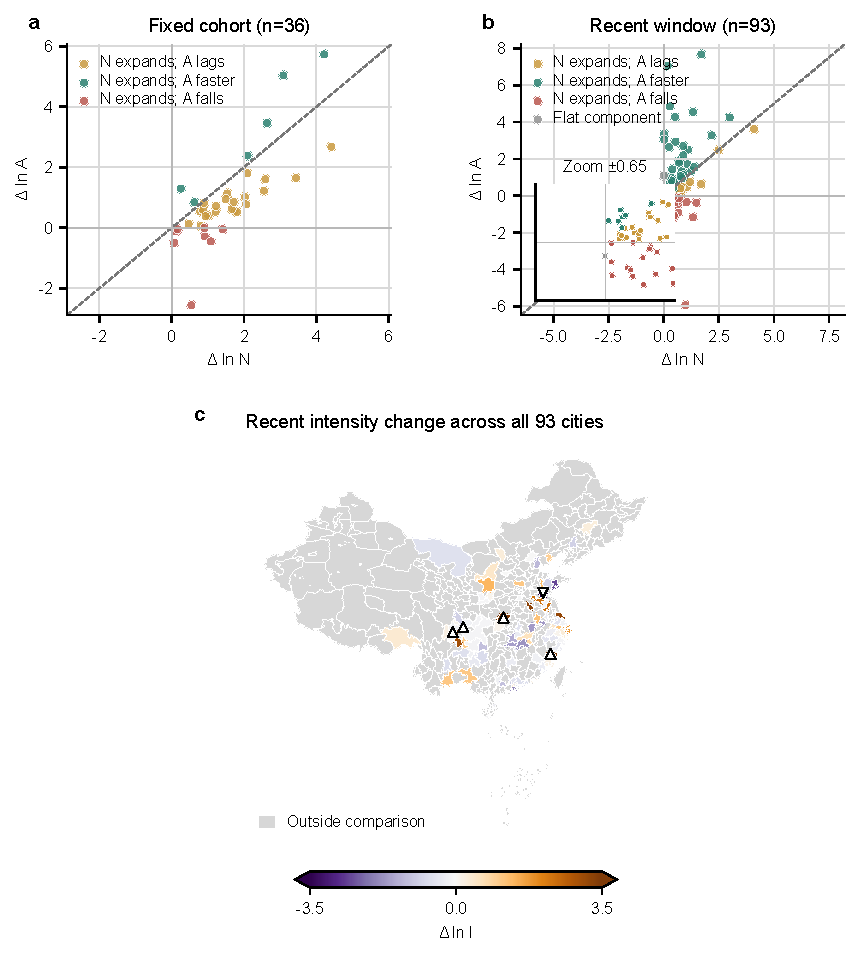
\includegraphics[width=\linewidth,height=.76\textheight,keepaspectratio]{figures/fig4_regimes.pdf}
\caption{City growth patterns by common window}\label{fig:regimes}
\end{figure}


The paired comparison adds temporal structure to these window-specific categories. In the primary non-overlapping 52-city comparison, 19 city pairs retain the same category (36.54\%). Among the 27 cities that were faster-growth in 2020--2021, 10 remain faster, 10 become slower-positive and 7 become contraction cases: 17 of 27 therefore change category. The three early contraction cases all show positive late activity growth, with one becoming faster-growth and two becoming slower-positive. Percentages are conditional on the early category; for example, the 10 faster-to-slower pairs are 37.04\% of that 27-city column, not of all 52 cities. The supplementary 73-city pairing retains 32 same-category pairs. SI Table~\siref{tab:growth_transition_details} gives both matrices, and SI Table~\siref{tab:growth_transition_other} identifies the Other subtypes.

The transition evidence is consequently about persistence and reclassification within observed cities, not a causal transition process. A favourable relative-growth category can be followed by slower growth or contraction, while an early contraction label does not fix the late category. The paired windows retain their stated observation rules and are interpreted alongside, rather than as a replacement for, the broader endpoint states (Figure~\ref{fig:transitions}).
\begin{figure}[htbp]\centering
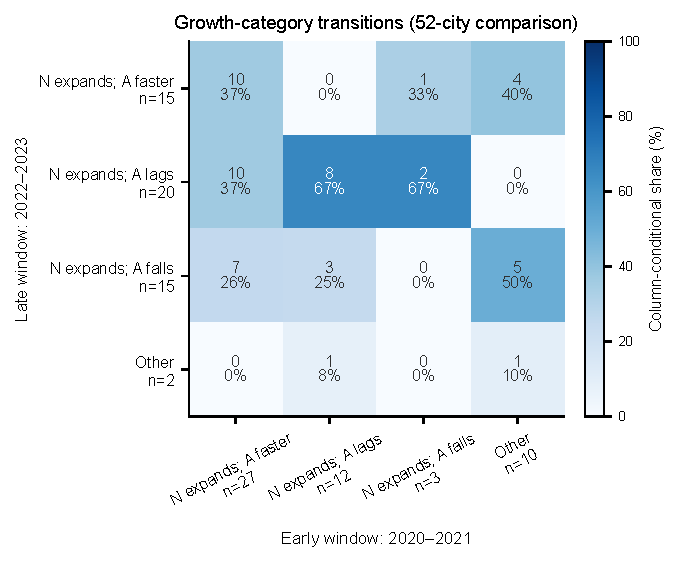
\includegraphics[width=\linewidth,height=.76\textheight,keepaspectratio]{figures/fig5_growth_transitions.pdf}
\caption{Growth regime transitions across matched cities}\label{fig:transitions}
\end{figure}

